\documentclass[14pt,a4paper]{extarticle}
\usepackage[utf8]{inputenc}
\usepackage[T2A]{fontenc}
\usepackage[russian]{babel}
\usepackage{geometry}
\usepackage{setspace}
\usepackage{indentfirst}
\usepackage{graphicx}
\usepackage{longtable}
\usepackage{enumitem}
\usepackage{mathptmx}

\geometry{left=30mm,right=10mm,top=20mm,bottom=20mm}
\setlength{\parindent}{1.25cm}
\onehalfspacing
\sloppy

\begin{document}

% -----------------------------
% Титульный лист
% -----------------------------
\begin{titlepage}
\begin{center}
Министерство науки и высшего образования Российской Федерации\\
НИЯУ МИФИ\\
Факультет ИИКС\\
Кафедра 22
\end{center}

\vfill

\begin{center}
\textbf{Лабораторная работа № 2}\\
\textbf{«Составление расписания с ограничениями»}\\
по дисциплине: Логическое программирование
\end{center}

\vfill

\begin{flushright}
Выполнил: студент Якименко Никита Валерьевич\\
Группа: Б24-517\\
Проверил: \underline{\hspace{6cm}}
\end{flushright}

\vfill

\begin{center}
г. Москва \hspace{1cm} 2026
\end{center}
\end{titlepage}

\tableofcontents
\newpage

% -----------------------------
% 1. Описание предметной области
% -----------------------------
\section{Описание предметной области}
Смоделировано расписание учебных занятий вымышленного потока из пяти групп
(\texttt{g101..g105}) на одну неделю (понедельник--пятница) с шестью временными
слотами в день. В расписании участвуют 10 предметов, 5 преподавателей и 10
аудиторий (включая компьютерные классы).

% -----------------------------
% 2. Схема БЗ и домены
% -----------------------------
\section{Схема БЗ (структура фактов и домены значений)}
База знаний реализована в Prolog. Основные факты:

\begin{itemize}[leftmargin=1.25cm]
  \item \texttt{group(Group, Size)} --- группы и численность.
  \item \texttt{subject(Subject)} --- предметы.
  \item \texttt{teacher(Teacher)} --- преподаватели.
  \item \texttt{room(Room, Capacity, Equipment)} --- аудитории, вместимость и оборудование.
  \item \texttt{subject\_req(Subject, Equipment)} --- требования предмета к оборудованию.
  \item \texttt{day(Day)} и \texttt{day\_index(Day, Index)} --- дни недели.
  \item \texttt{slot\_time(Slot, Time)} --- расписание временных слотов.
  \item \texttt{занятие(Group, Subject, Teacher, Day, Slot, Room)} --- занятия в БЗ.
\end{itemize}

Домены значений:
\begin{itemize}[leftmargin=1.25cm]
  \item \texttt{Day} $\in$ \{mon, tue, wed, thu, fri\}.
  \item \texttt{Slot} $\in$ \{1..6\}.
  \item \texttt{Room} $\in$ \{r101, r102, r103, r201, r202, r203, lab1, lab2, aud1, aud2\}.
  \item оборудование: \texttt{pc}, \texttt{projector}.
\end{itemize}

% -----------------------------
% 3. Реализованные запросы
% -----------------------------
\section{Реализованные запросы (примеры работы)}
Ниже приведены примеры запросов и полученные результаты (SWI-Prolog).

\subsection*{Пример 1. Когда у группы g101 предмет math?}
\begin{verbatim}
?- когда_у_группы(g101, math, Day, Slot, Room).
Day = mon, Slot = 1, Room = r101.
\end{verbatim}

\subsection*{Пример 2. Какие аудитории свободны в среду в 10:40 (slot 2)?}
\begin{verbatim}
?- свободна_аудитория(wed, 2, Room).
Room = [r101,r102,r103,r201,r202,r203,lab2,aud1,aud2].
\end{verbatim}

\subsection*{Пример 3. У каких групп занятия ведет преподаватель petrov?}
\begin{verbatim}
?- группы_преподавателя(petrov, Groups).
Groups = [g101,g102,g103,g104,g105].
\end{verbatim}

\subsection*{Пример 4. Сколько пар в неделю у группы g102?}
\begin{verbatim}
?- нагрузка_группы(g102, Count).
Count = 6.
\end{verbatim}

\subsection*{Пример 5. Свободные дни преподавателя orlova}
\begin{verbatim}
?- свободные_дни_преподавателя(orlova, Days).
Days = [tue,wed,thu].
\end{verbatim}

\subsection*{Пример 6. Окна в расписании группы g101}
\begin{verbatim}
?- окна_в_расписании(g101, Windows).
Windows = 2.
\end{verbatim}

\subsection*{Пример 7. День с минимальной нагрузкой для g104}
\begin{verbatim}
?- день_с_минимальной_нагрузкой(g104, Day).
Day = mon.
\end{verbatim}

% -----------------------------
% 4. Уровень 2: Валидация
% -----------------------------
\section{Уровень 2: Валидация и метрики}
Реализованы проверки корректности расписания:
\begin{itemize}[leftmargin=1.25cm]
  \item \texttt{нет\_конфликтов\_групп/0}.
  \item \texttt{нет\_конфликтов\_преподавателей/0}.
  \item \texttt{нет\_конфликтов\_аудиторий/0} (вместимость и оборудование).
\end{itemize}

Результаты валидации:
\begin{verbatim}
?- нет_конфликтов_групп,
   нет_конфликтов_преподавателей,
   нет_конфликтов_аудиторий.
true.
\end{verbatim}

Перегруженные преподаватели (более 20 часов в неделю) отсутствуют:
\begin{verbatim}
?- перегруженные_преподаватели(Teachers).
Teachers = [].
\end{verbatim}

% -----------------------------
% 5. Уровень 3: CLP(FD)
% -----------------------------
\section{Уровень 3: Генерация расписания (CLP(FD))}
Для автоматической генерации используется библиотека \texttt{clpfd}.

\subsection*{Входные данные}
Учебный план и закрепление преподавателей задаются фактами:
\begin{verbatim}
requirement(Group, Subject, Pairs).
teacher_for(Group, Subject, Teacher).
\end{verbatim}

\subsection*{Ограничения}
\begin{itemize}[leftmargin=1.25cm]
  \item 5 дней $\times$ 6 пар = 30 слотов.
  \item отсутствие конфликтов для групп, преподавателей, аудиторий.
  \item соответствие вместимости и оборудования аудитории.
  \item равномерная нагрузка: не более 3 пар в день, разброс по дням не более 2.
  \item минимизация окон в расписании (целевой критерий).
\end{itemize}

\subsection*{Запуск генератора}
\begin{verbatim}
?- генерировать_расписание(Schedule), length(Schedule, Len).
Len = 30.
\end{verbatim}

\subsection*{Скриншот сгенерированного расписания}
\begin{figure}[h!]
\centering
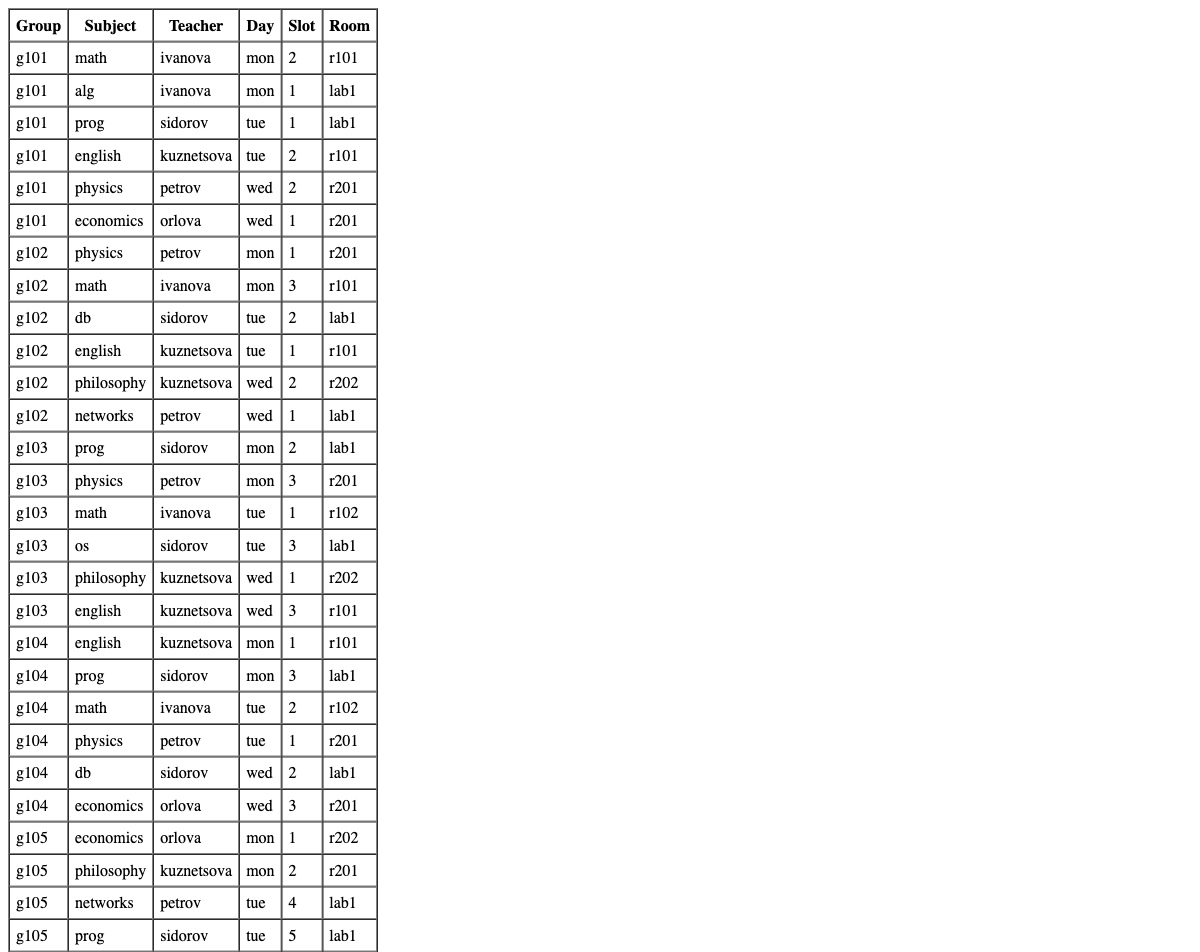
\includegraphics[width=\textwidth]{output/playwright/schedule.png}
\caption{Скриншот HTML-расписания, сгенерированного CLP(FD)}
\end{figure}

% -----------------------------
% 6. Экспорт и файлы
% -----------------------------
\section{Экспорт расписания}
Экспорт выполнен в CSV и HTML:
\begin{verbatim}
generated_schedule.csv
generated_schedule.html
\end{verbatim}

\section*{Заключение}
Построена база знаний расписания и реализованы запросы анализа. Добавлена
валидация расписания и генератор с ограничениями CLP(FD), обеспечивающий
корректность и оптимизацию по числу окон. Расписание экспортируется в табличный
формат для дальнейшего использования.

\end{document}
